\subsection{Preliminary Results}

\label{sec:results}

\begin{frame}{Datasets}	
	We use Oxford RobotCar dataset \cite{Maddern2016} as it includes:
	\begin{itemize}
		\item Time redundancy for each car trajectory
		\item 4 cameras on the car \& 3 LIDARS (3 modalities: RGB, Depth \& Reflectance)
	\end{itemize}
	\vfill
	\begin{minipage}[c]{0.22\linewidth}
		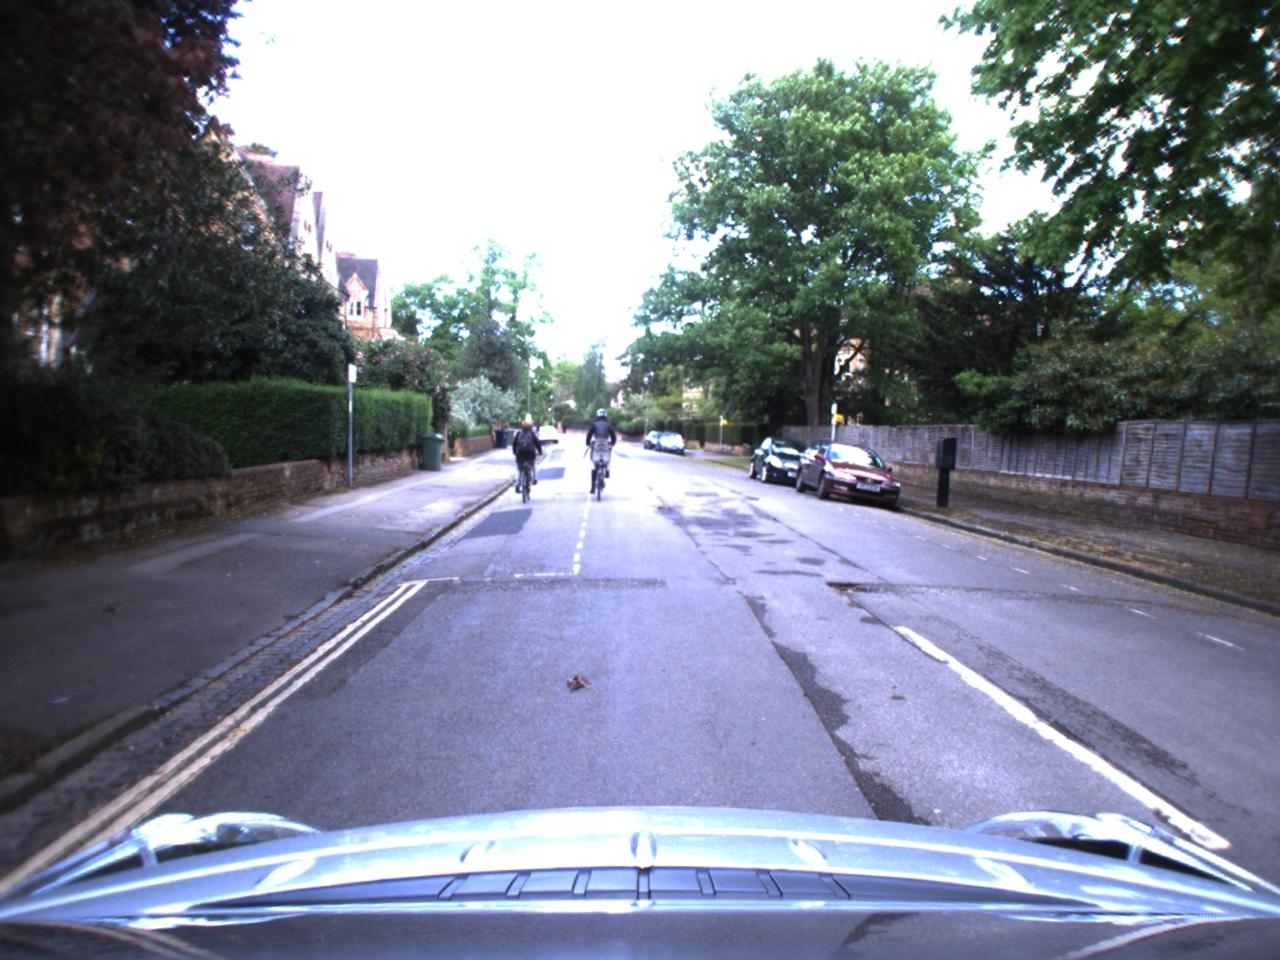
\includegraphics[width=\linewidth]{images/robotcar_1.jpg}
		
		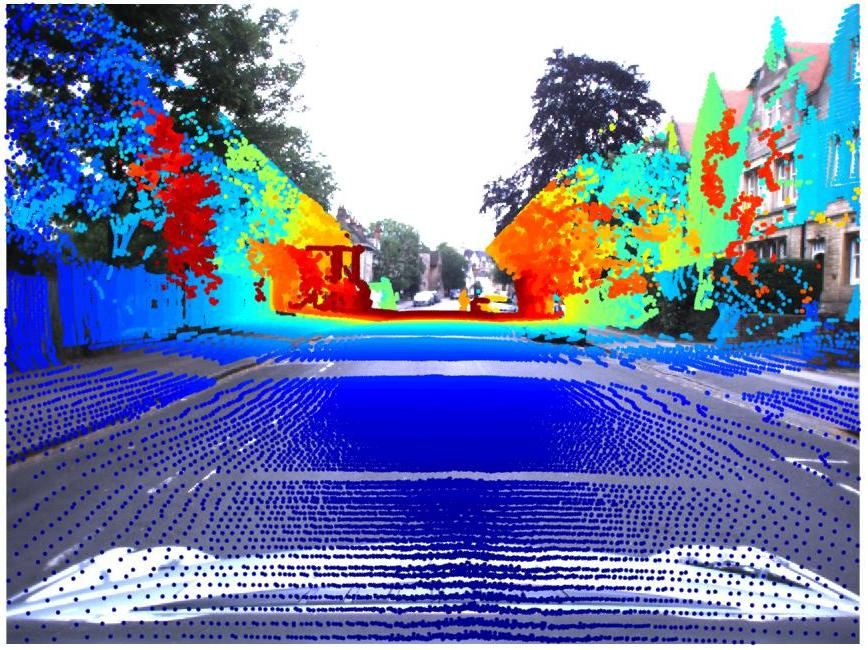
\includegraphics[width=\linewidth]{images/robotcar_depth.jpg}	
	\end{minipage}
	\hfill					
	\begin{minipage}[c]{0.77\linewidth}
		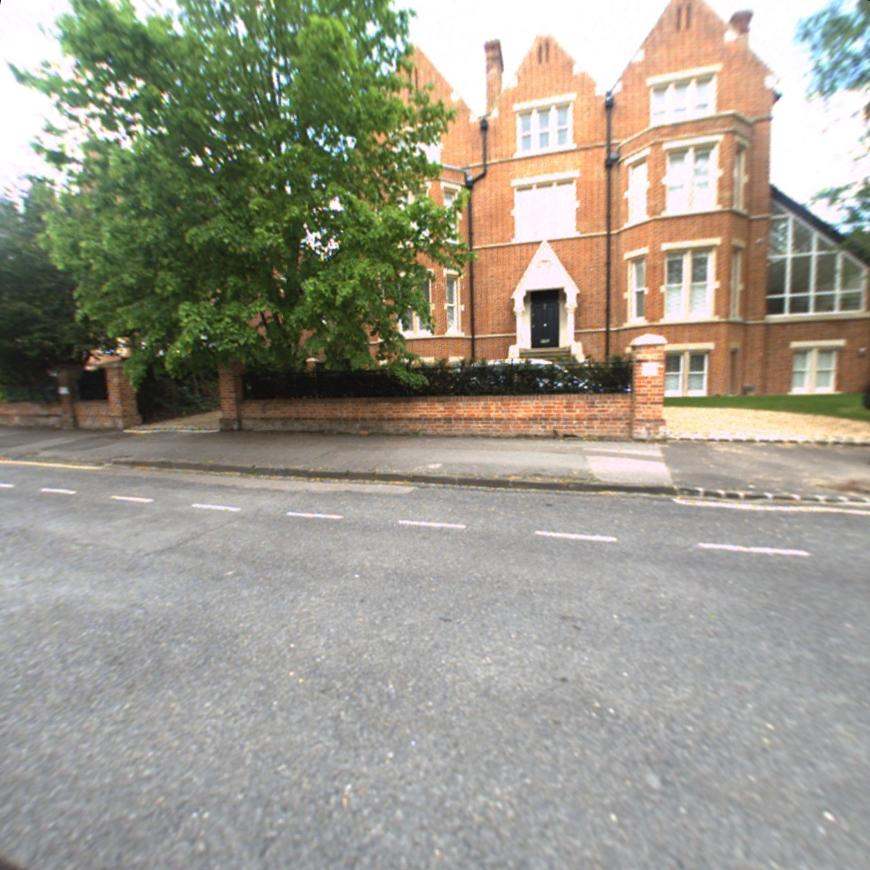
\includegraphics[width=0.3\linewidth]{images/robotcar_2.jpg}\hfill					
		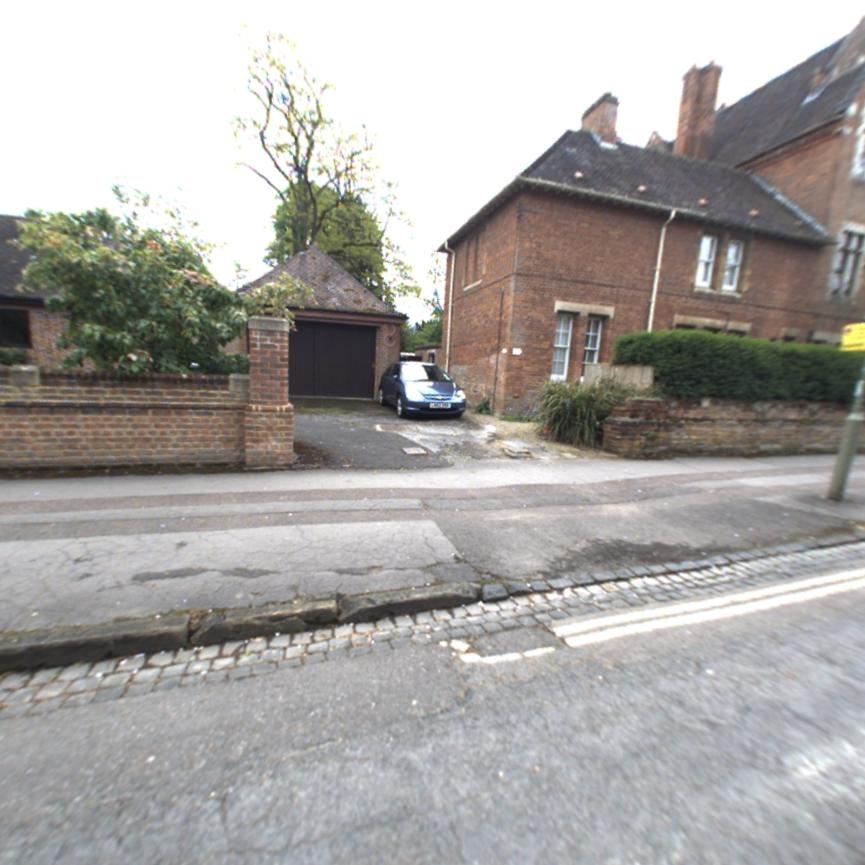
\includegraphics[width=0.3\linewidth]{images/robotcar_3.jpg}\hfill					
		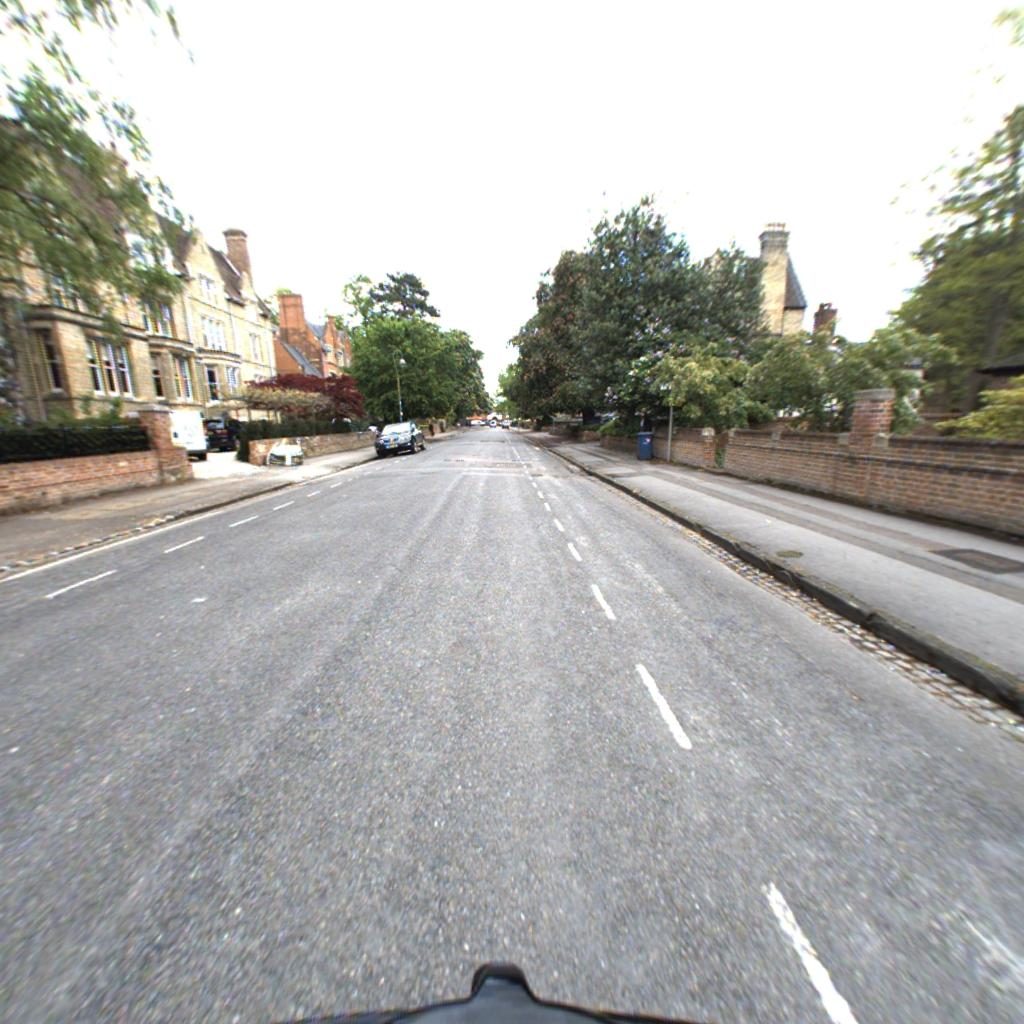
\includegraphics[width=0.3\linewidth]{images/robotcar_4.jpg}					
	\end{minipage}
\end{frame}

\newlength{\widthcase}
\setlength{\widthcase}{2.4cm}
\begin{frame}{Data}
	\begin{tabular}{c c c c}
		\footnotesize{RGB} & \footnotesize{Raw depth} & \footnotesize{Regularized depth} & \footnotesize{Regularized reflectance} \\
		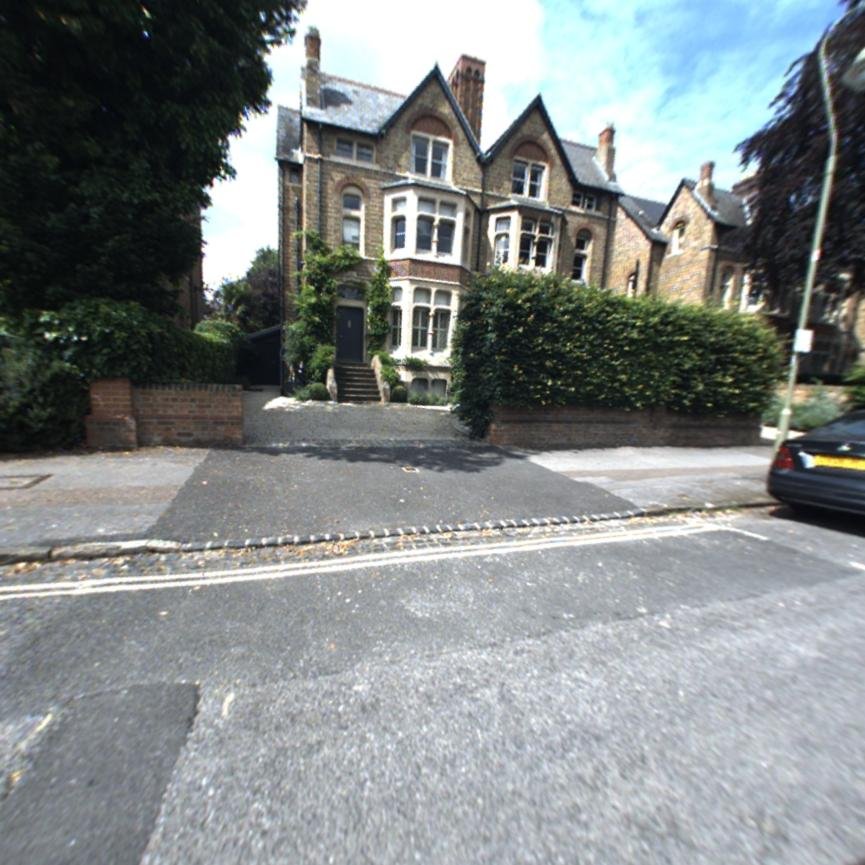
\includegraphics[width=\widthcase]{images/dataset/image_000052_mono_left.jpg} & 
		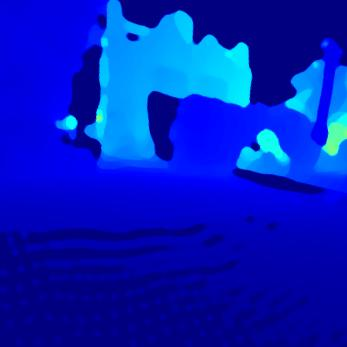
\includegraphics[width=\widthcase]{images/dataset/poordepth_000052_mono_left.jpg} &
		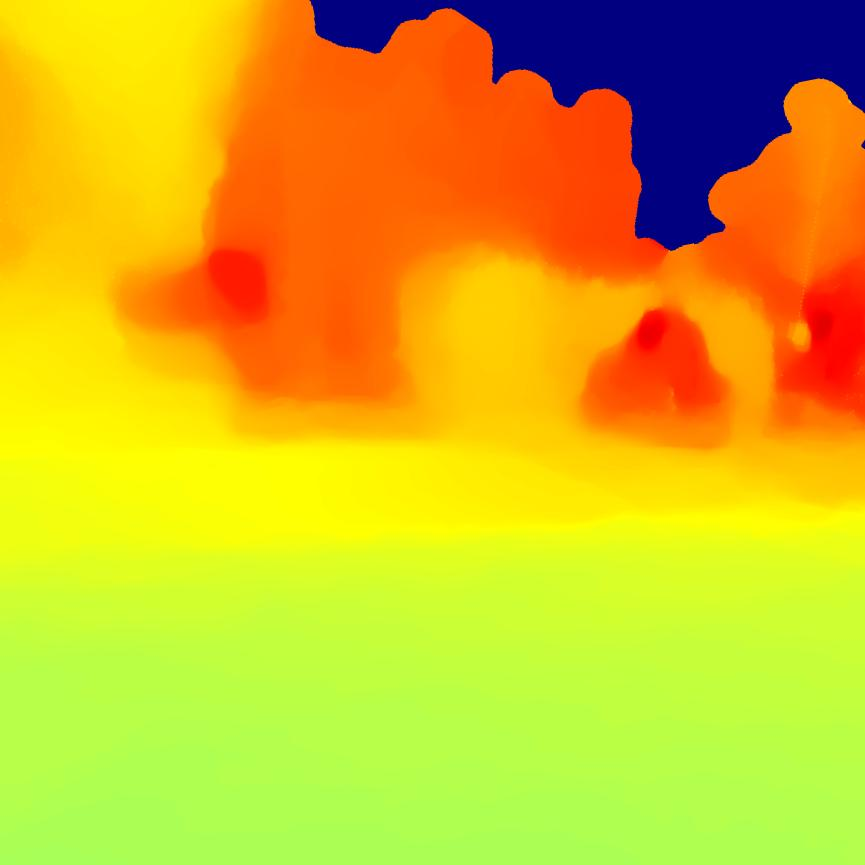
\includegraphics[width=\widthcase]{images/dataset/depth_000052_mono_left.jpg} &
		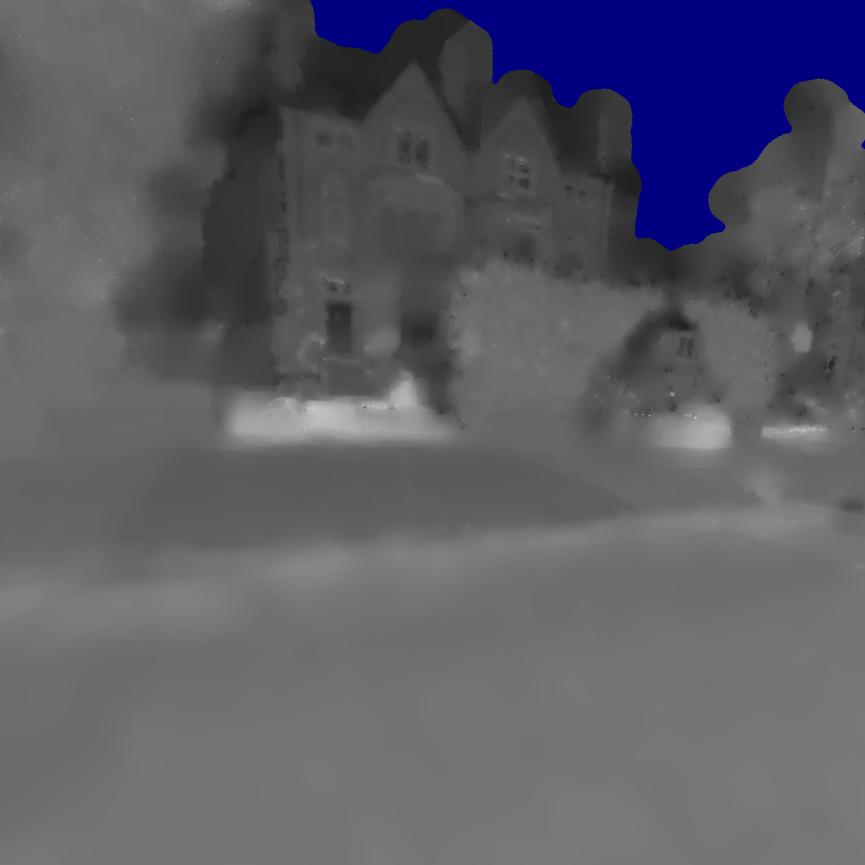
\includegraphics[width=\widthcase]{images/dataset/ref_000052_mono_left.jpg} \\
		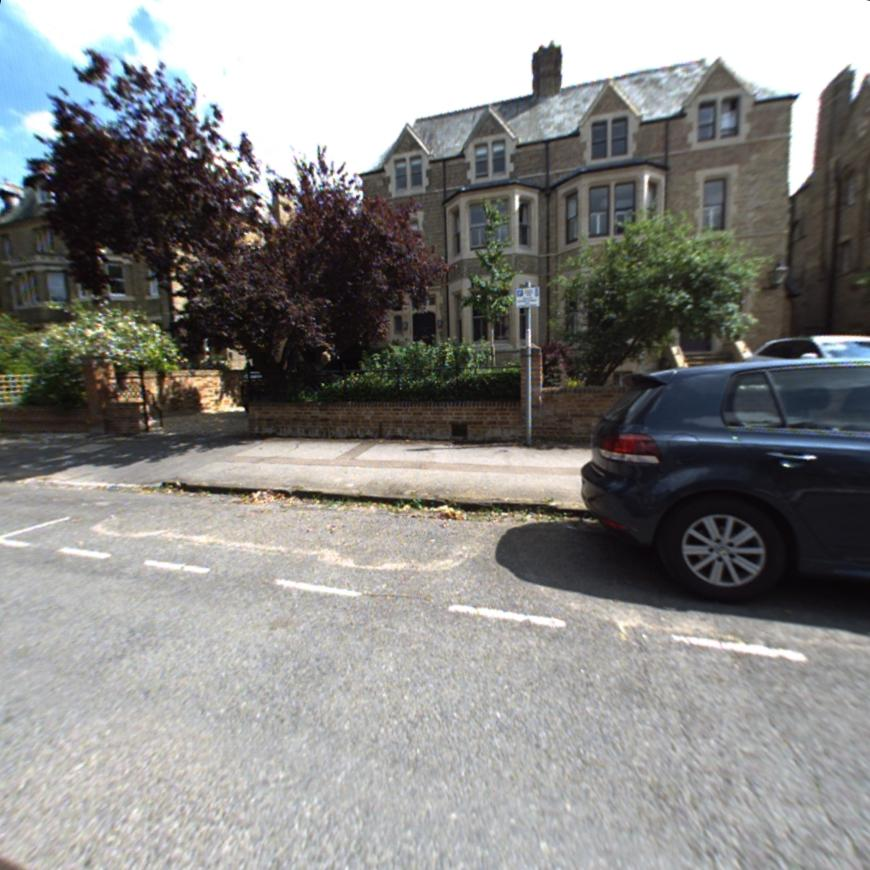
\includegraphics[width=\widthcase]{images/dataset/image_000052_mono_right.jpg} & 
		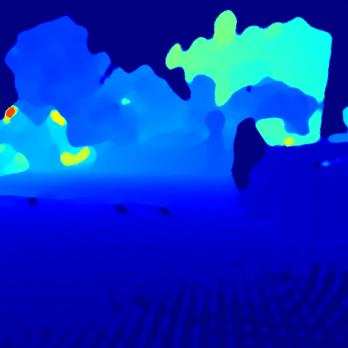
\includegraphics[width=\widthcase]{images/dataset/poordepth_000052_mono_right.jpg} &
		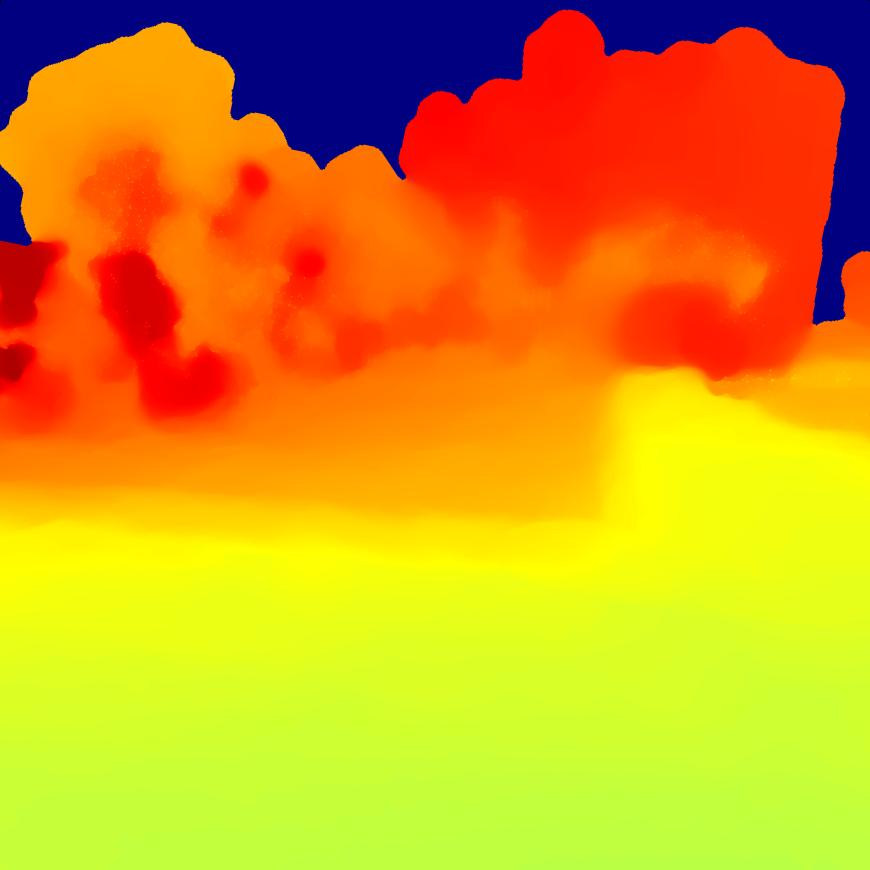
\includegraphics[width=\widthcase]{images/dataset/depth_000052_mono_right.jpg} &
		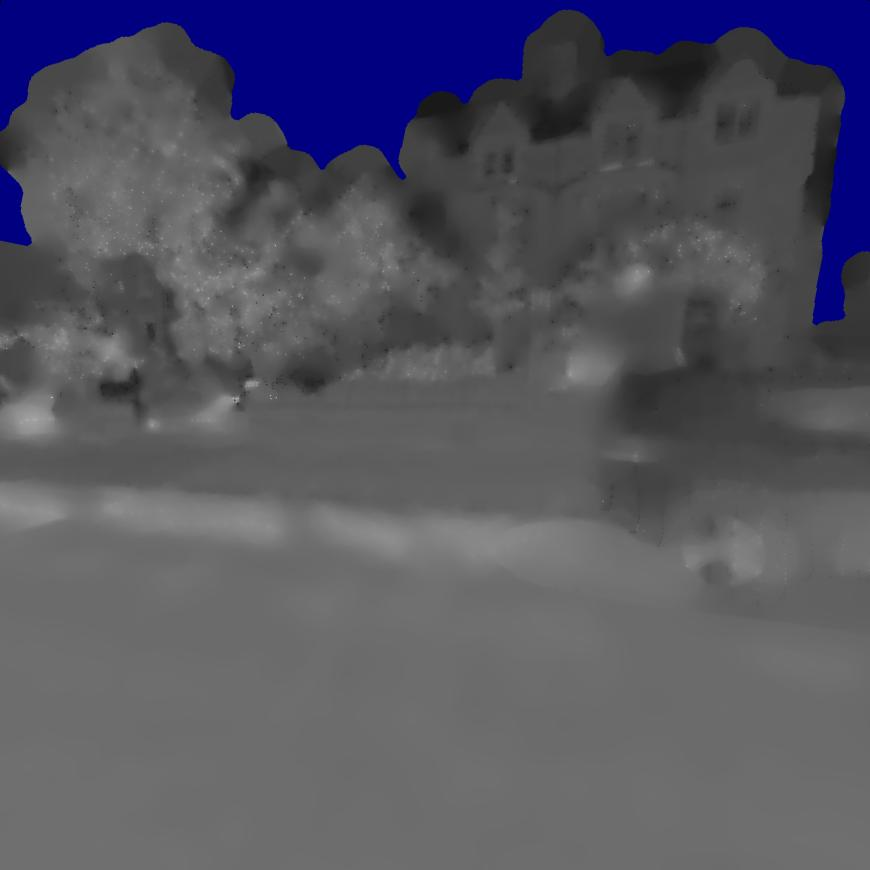
\includegraphics[width=\widthcase]{images/dataset/ref_000052_mono_right.jpg} \\
	\end{tabular}
	\vfill
	Post-processing algorithm from \cite{Bevilacqua2017}.
\end{frame}

\begin{frame}{Data}
	\begin{tabular}{c c c c}
		\footnotesize{RGB} & \footnotesize{Raw depth} & \footnotesize{Regularized depth} & \footnotesize{Regularized reflectance} \\
		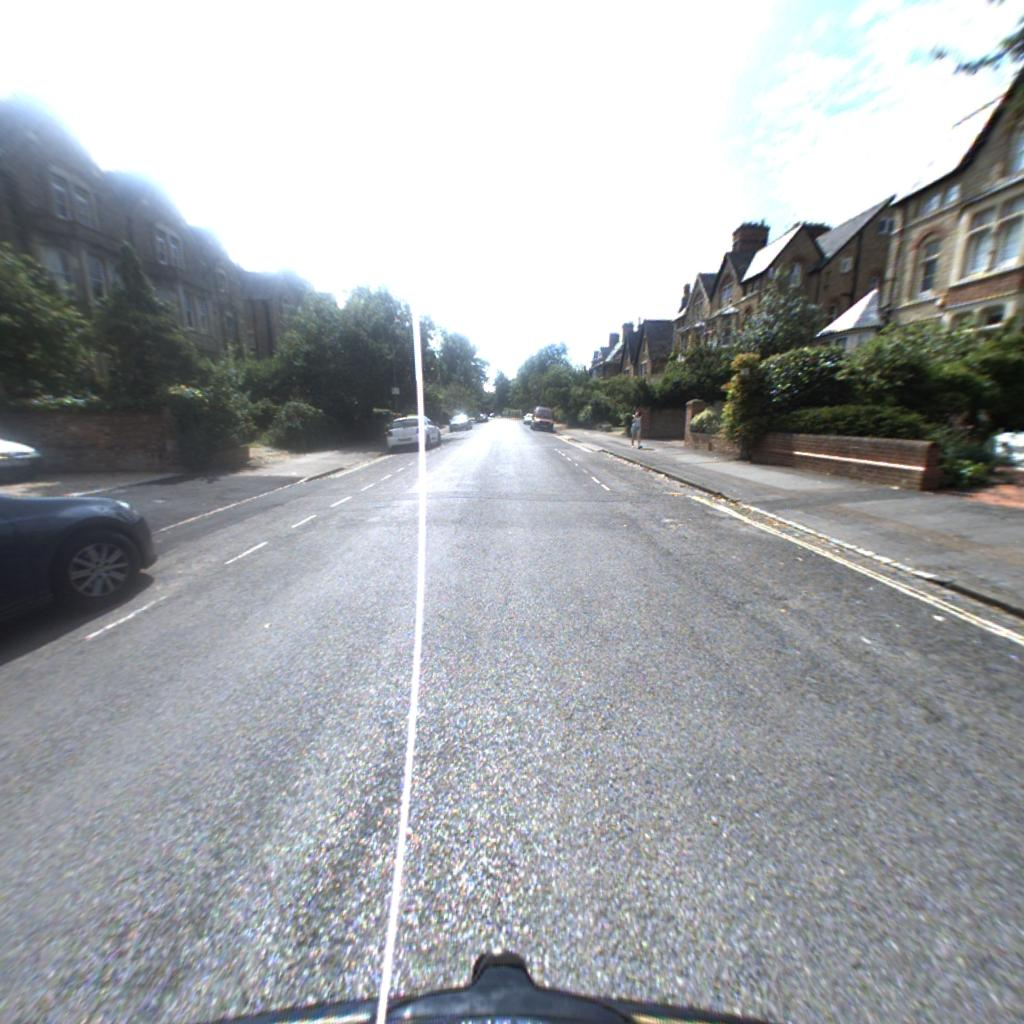
\includegraphics[width=\widthcase]{images/dataset/image_000052_mono_rear.jpg} & 
		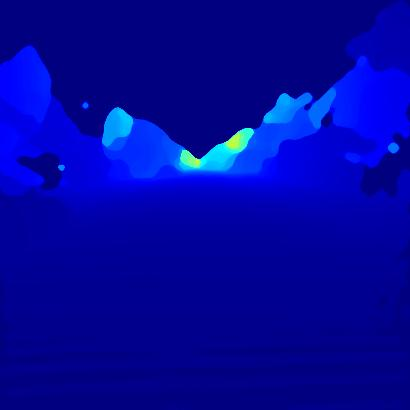
\includegraphics[width=\widthcase]{images/dataset/poordepth_000052_mono_rear.jpg} &
		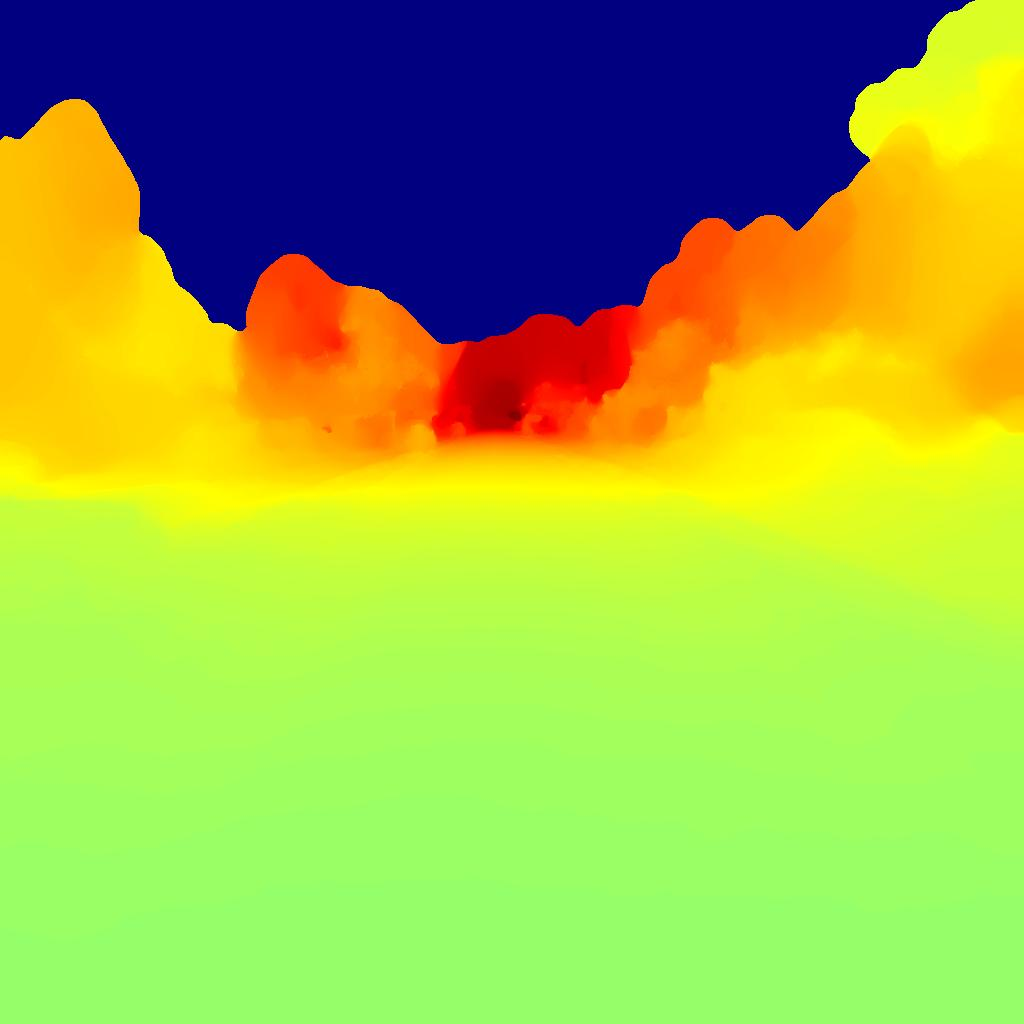
\includegraphics[width=\widthcase]{images/dataset/depth_000052_mono_rear.jpg} &
		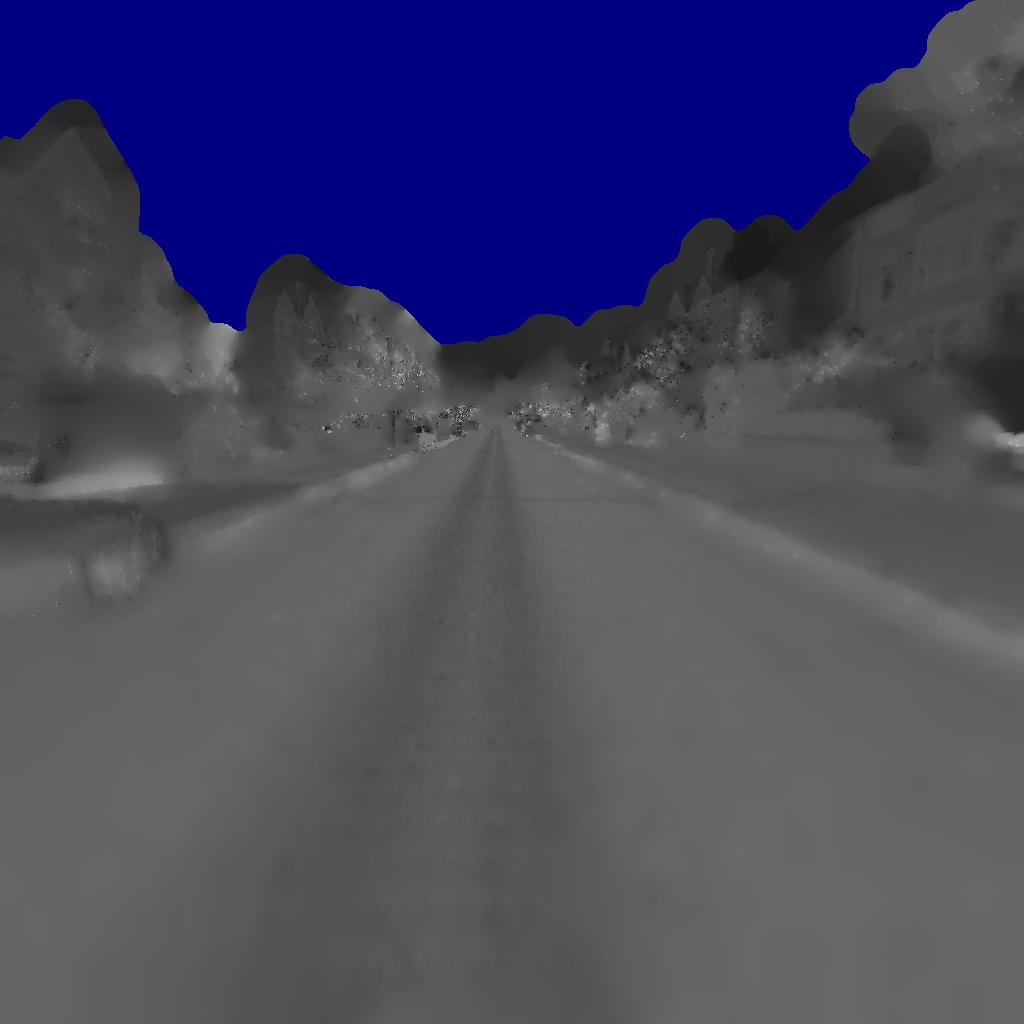
\includegraphics[width=\widthcase]{images/dataset/ref_000052_mono_rear.jpg} \\
		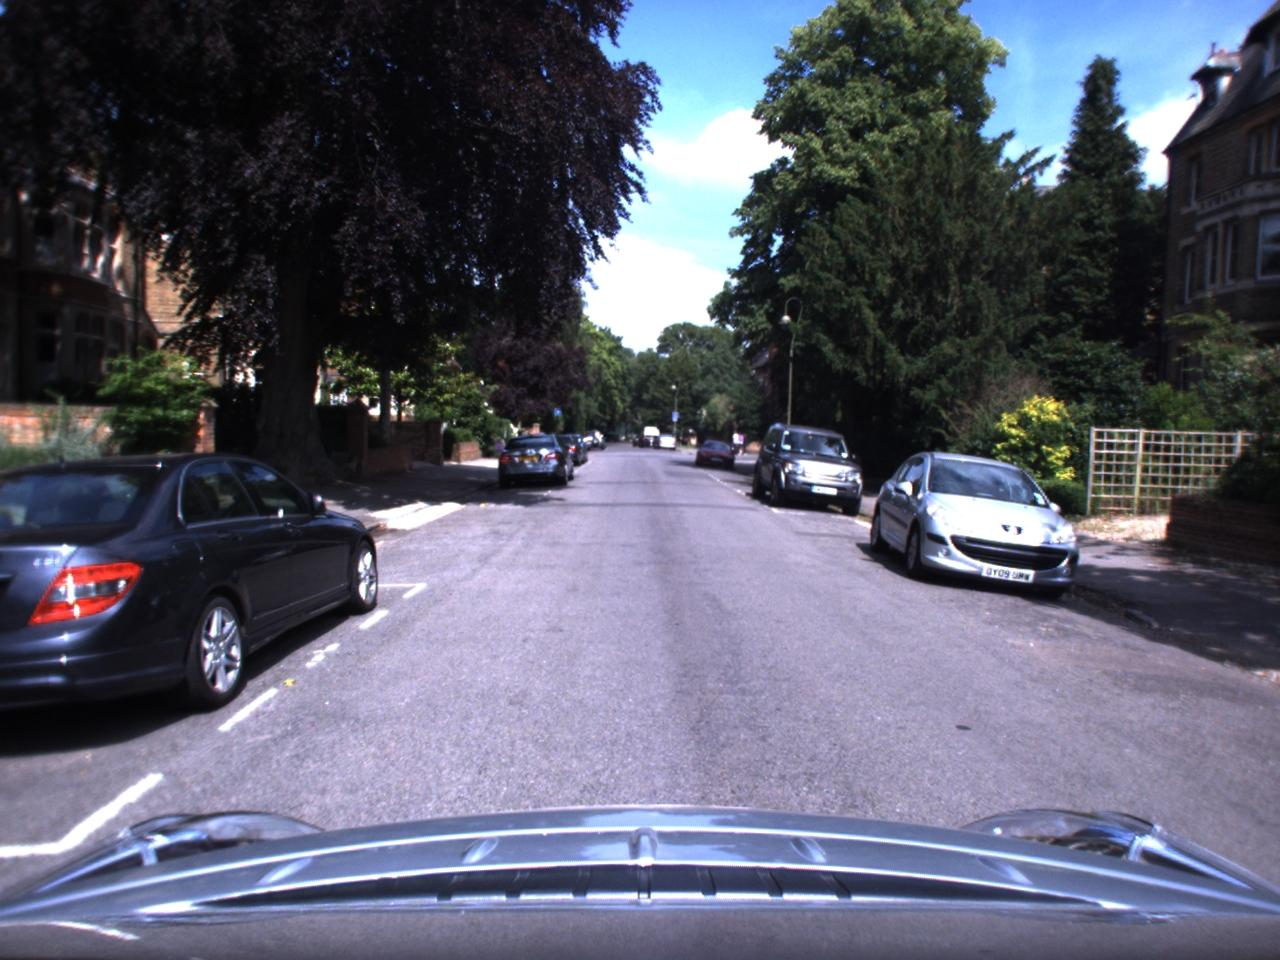
\includegraphics[width=\widthcase]{images/dataset/image_000052_stereo_centre.jpg} & 
		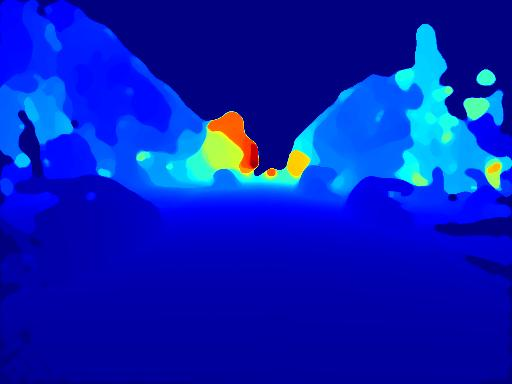
\includegraphics[width=\widthcase]{images/dataset/poordepth_000052_stereo_centre.jpg} &
		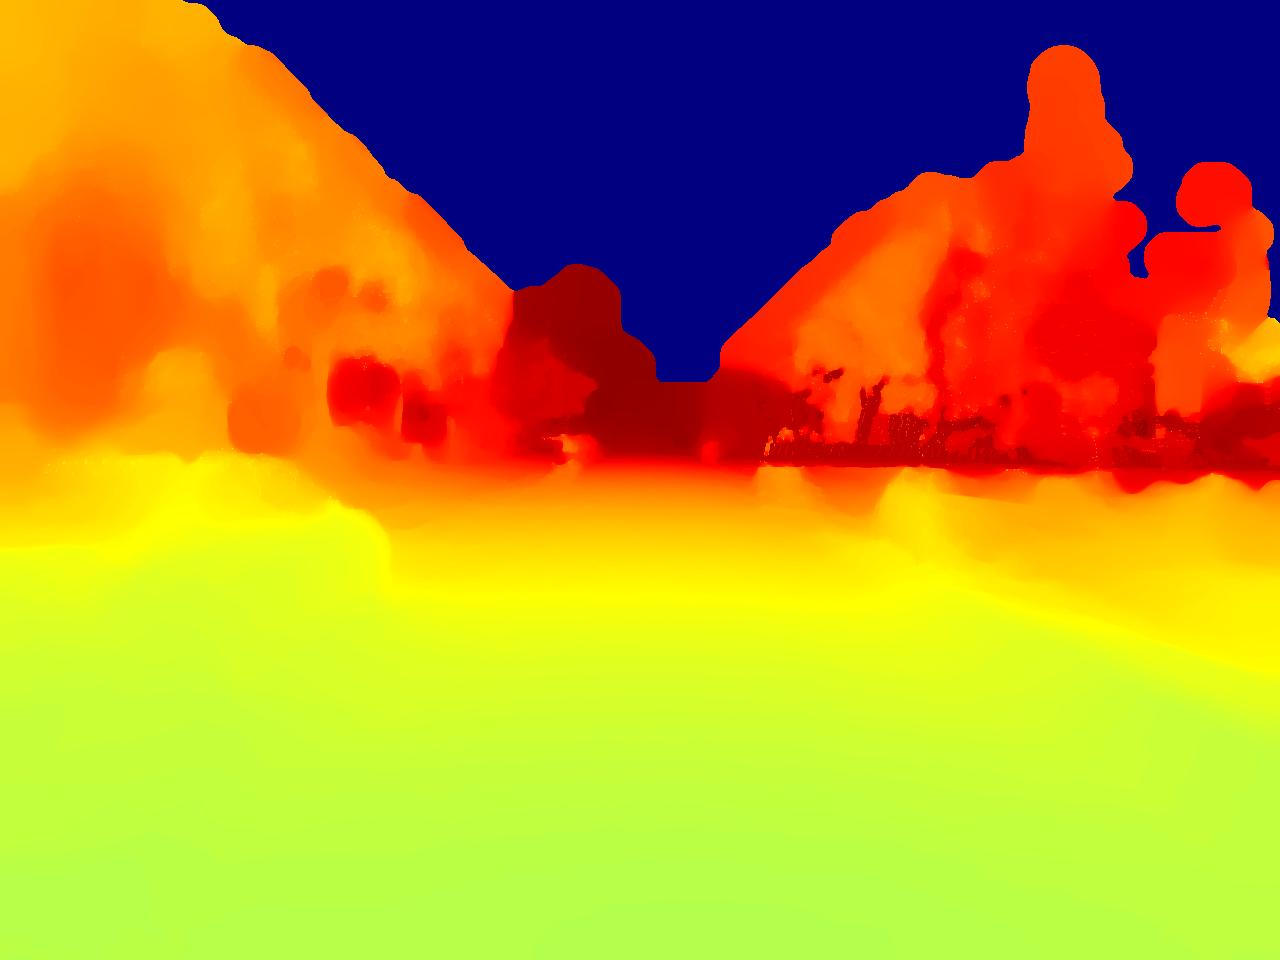
\includegraphics[width=\widthcase]{images/dataset/depth_000052_stereo_centre.jpg} &
		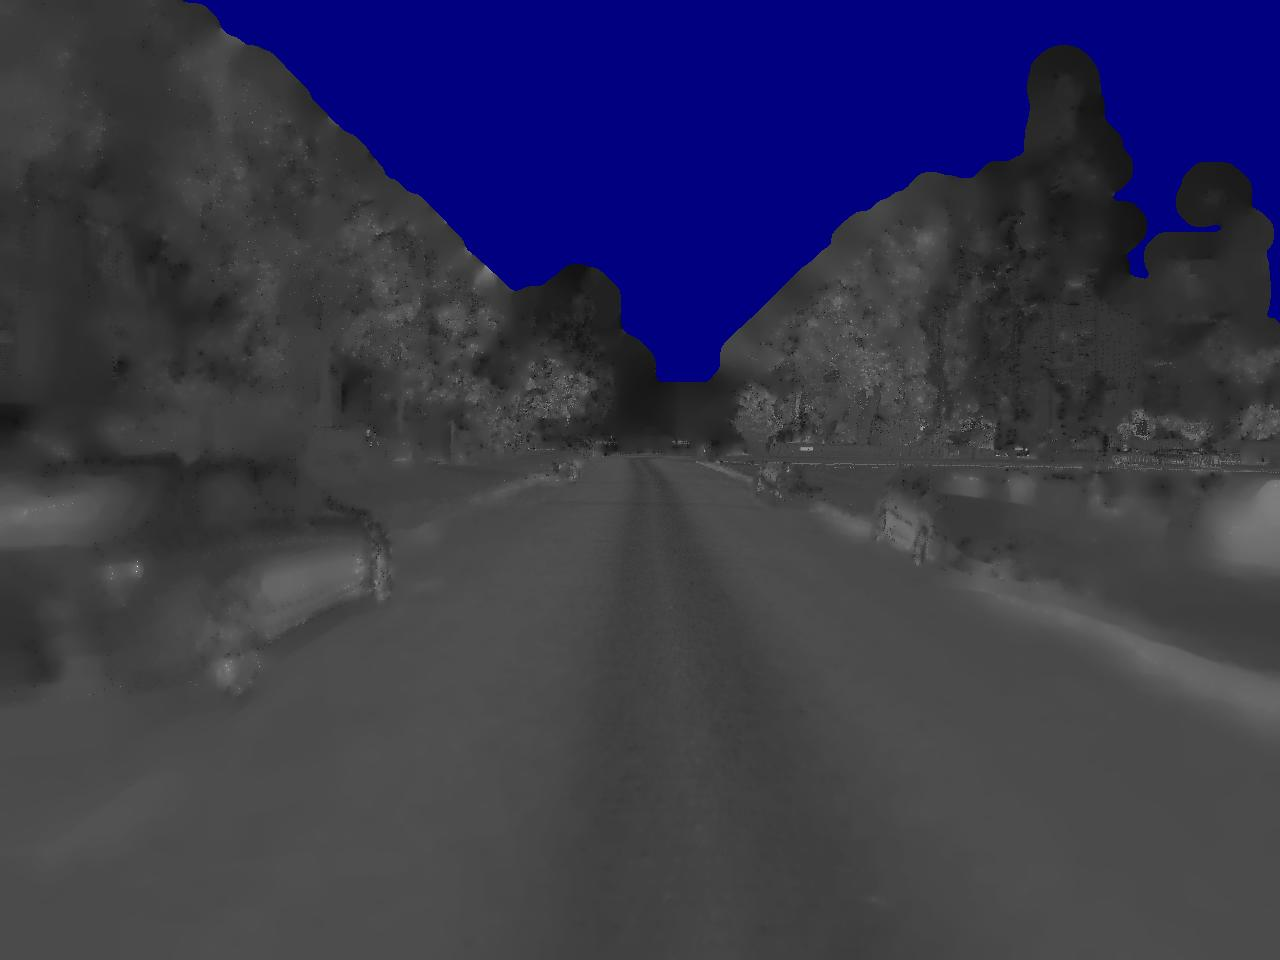
\includegraphics[width=\widthcase]{images/dataset/ref_000052_stereo_centre.jpg} \\		
	\end{tabular}
	\vfill
	Data are not perfect...
\end{frame}

\begin{frame}{Implementation details}
	\begin{itemize}
		\item[] \textbf{Deep Learning framework:} Pytorch
		\item[] \textbf{Coder net architecture:} Alexnet
		\item[] \textbf{Size of the training dataset:} 200 triplets (200 * 3 images * 2 modalities)
	\end{itemize}
	
	Trainings and validation frames are from a different region of Oxford than testing images.
\end{frame}

\begin{frame}{Does the transfer learning work?}
	\begin{minipage}[c]{0.24\linewidth}
		\begin{figure}[c]
			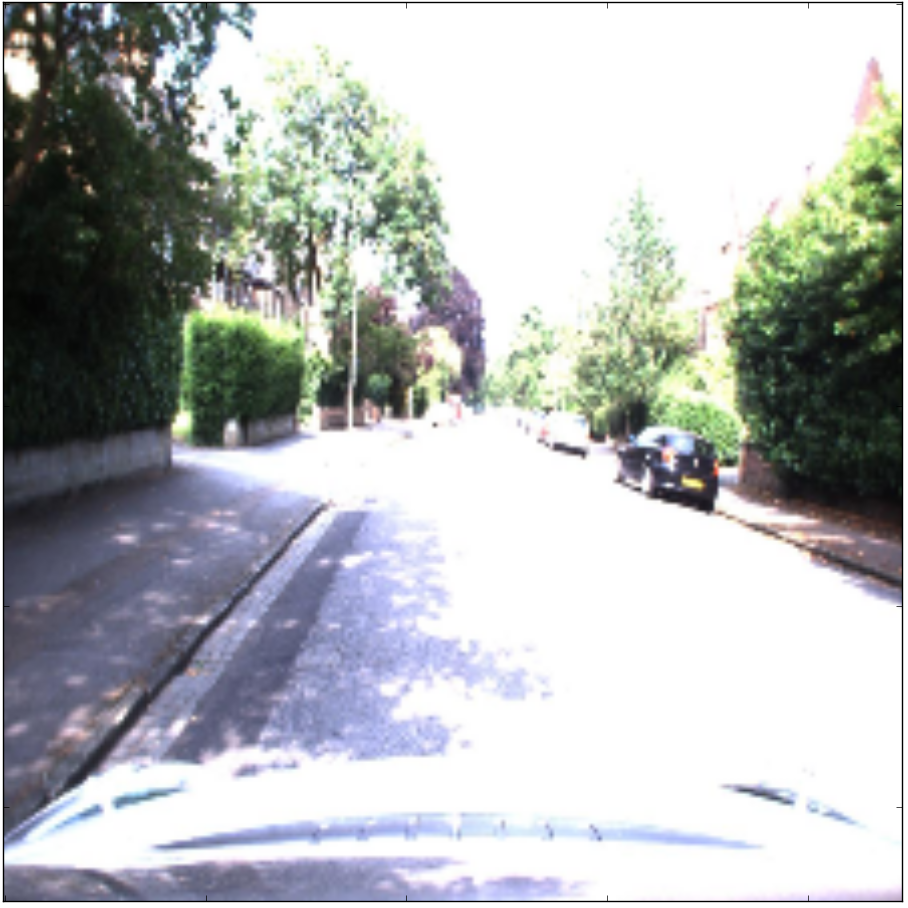
\includegraphics[width=0.5\linewidth]{images/rgb2.png}
		
			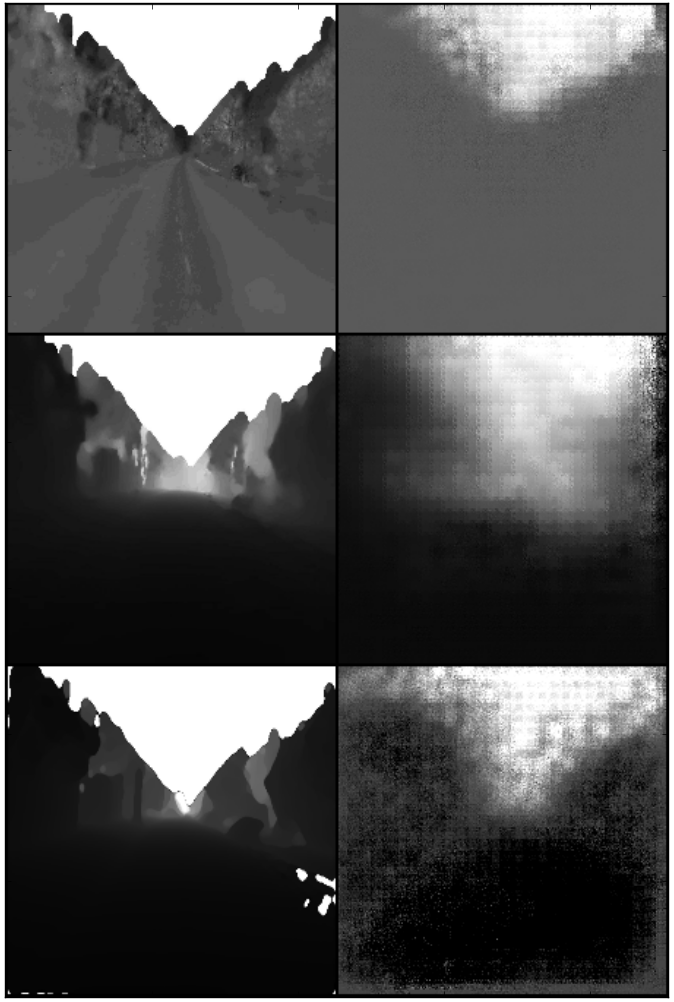
\includegraphics[width=\linewidth]{images/mod2.png}			
		\end{figure}
	\end{minipage}
	\hfill
	\begin{minipage}[c]{0.24\linewidth}
		\begin{figure}[c]
			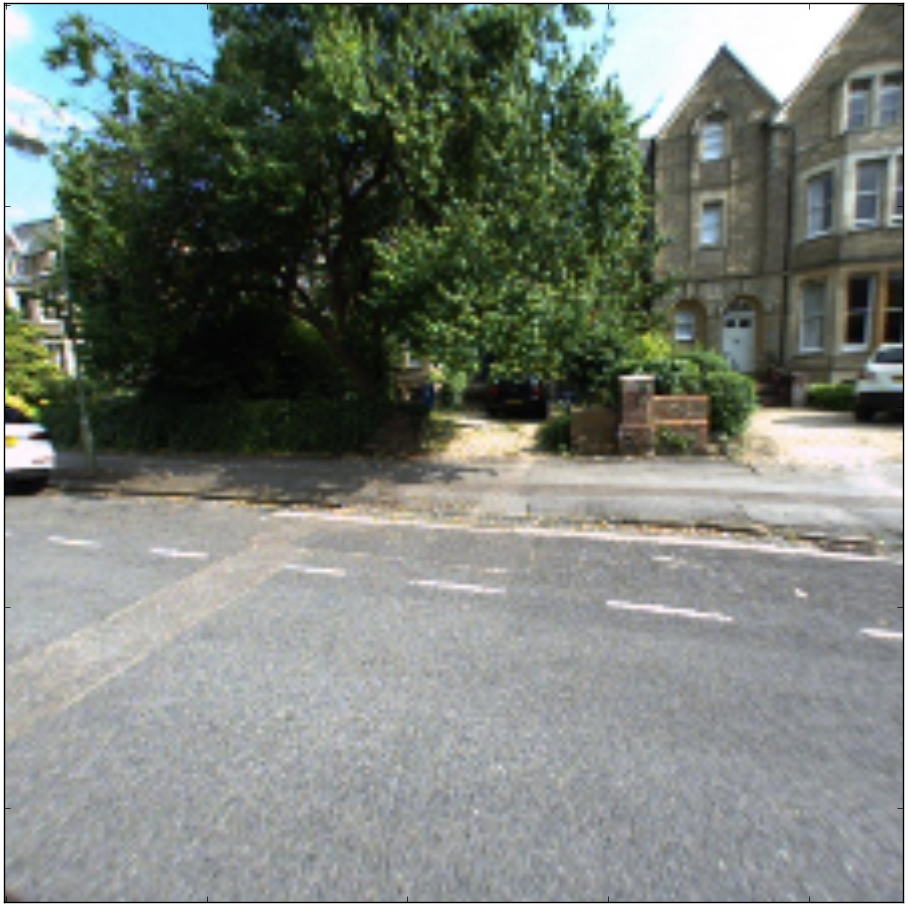
\includegraphics[width=0.5\linewidth]{images/rgb3.png}
		
			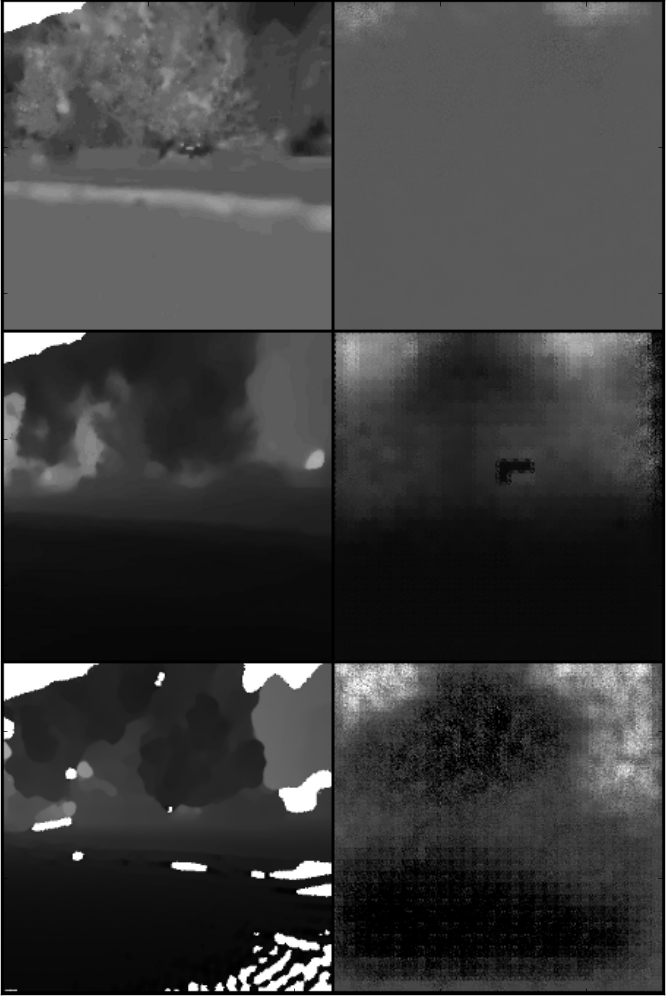
\includegraphics[width=\linewidth]{images/mod3.png}			
		\end{figure}
	\end{minipage}
	\hfill
	\begin{minipage}[c]{0.24\linewidth}
		\begin{figure}[c]
			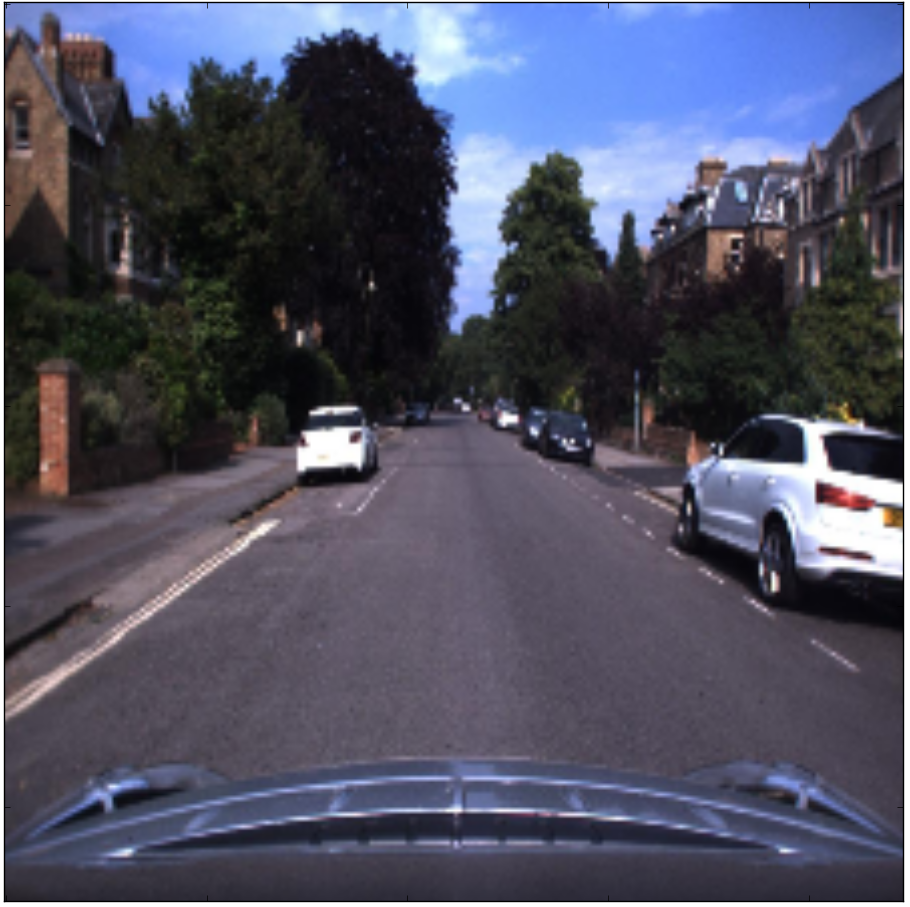
\includegraphics[width=0.5\linewidth]{images/rgb4.png}
		
			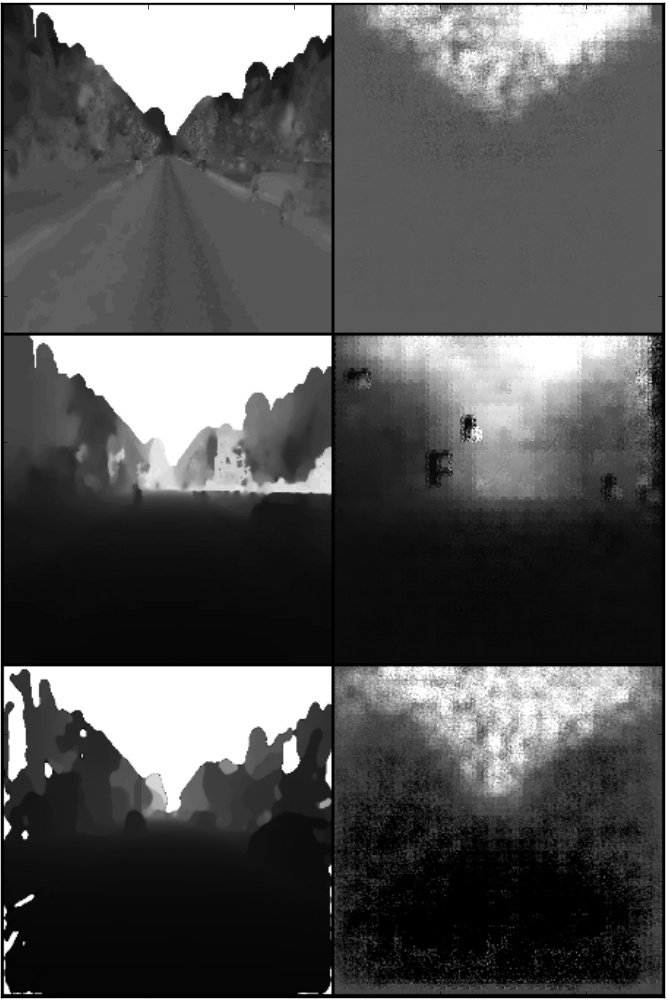
\includegraphics[width=\linewidth]{images/mod4.png}			
		\end{figure}
	\end{minipage}
	\hfill
	\begin{minipage}[c]{0.24\linewidth}
		\begin{figure}[c]
			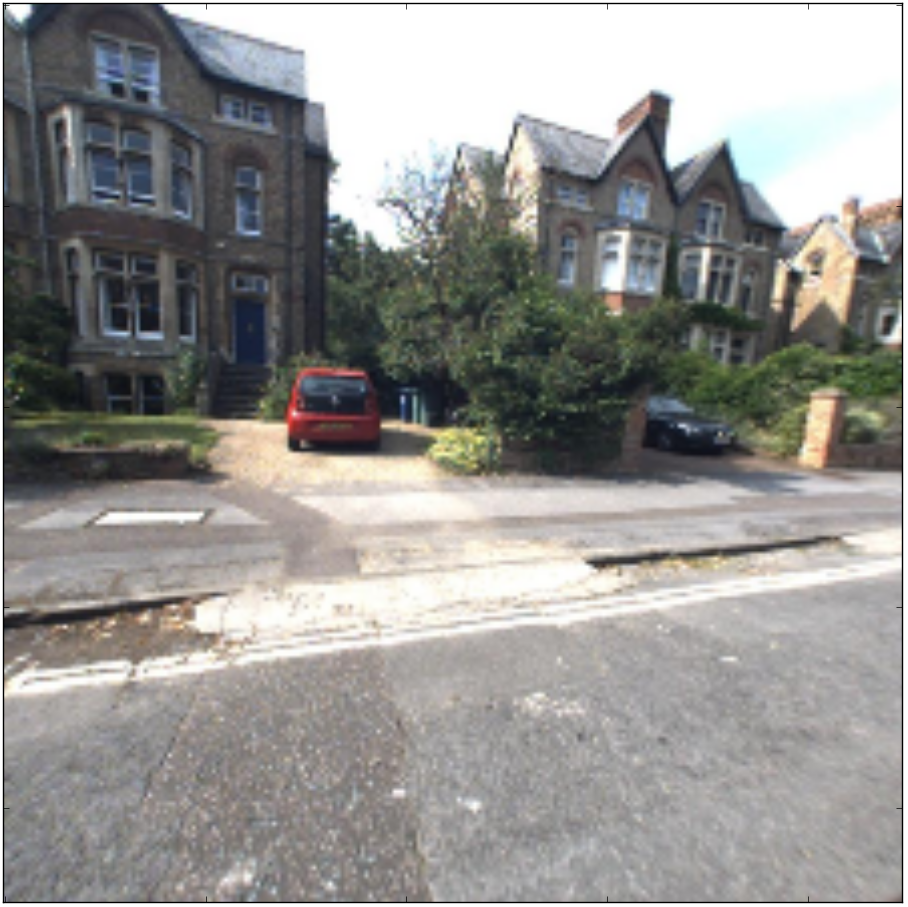
\includegraphics[width=0.5\linewidth]{images/rgb5.png}
		
			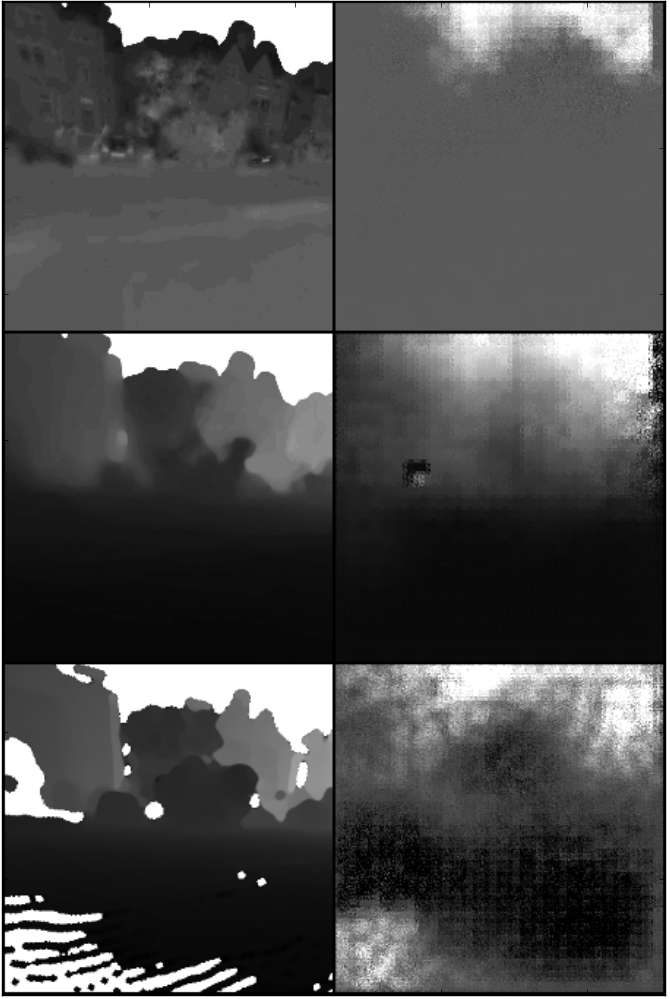
\includegraphics[width=\linewidth]{images/mod5.png}			
		\end{figure}
	\end{minipage}
\end{frame}

\begin{frame}{Does it improve the localization result?}
	\begin{block}{Evaluation}
		We state a query as registered if on of the top $K$ retrieved images is at a distance inferior at 25 metres. 
	\end{block}
	\vfill
	\begin{figure}[c]
		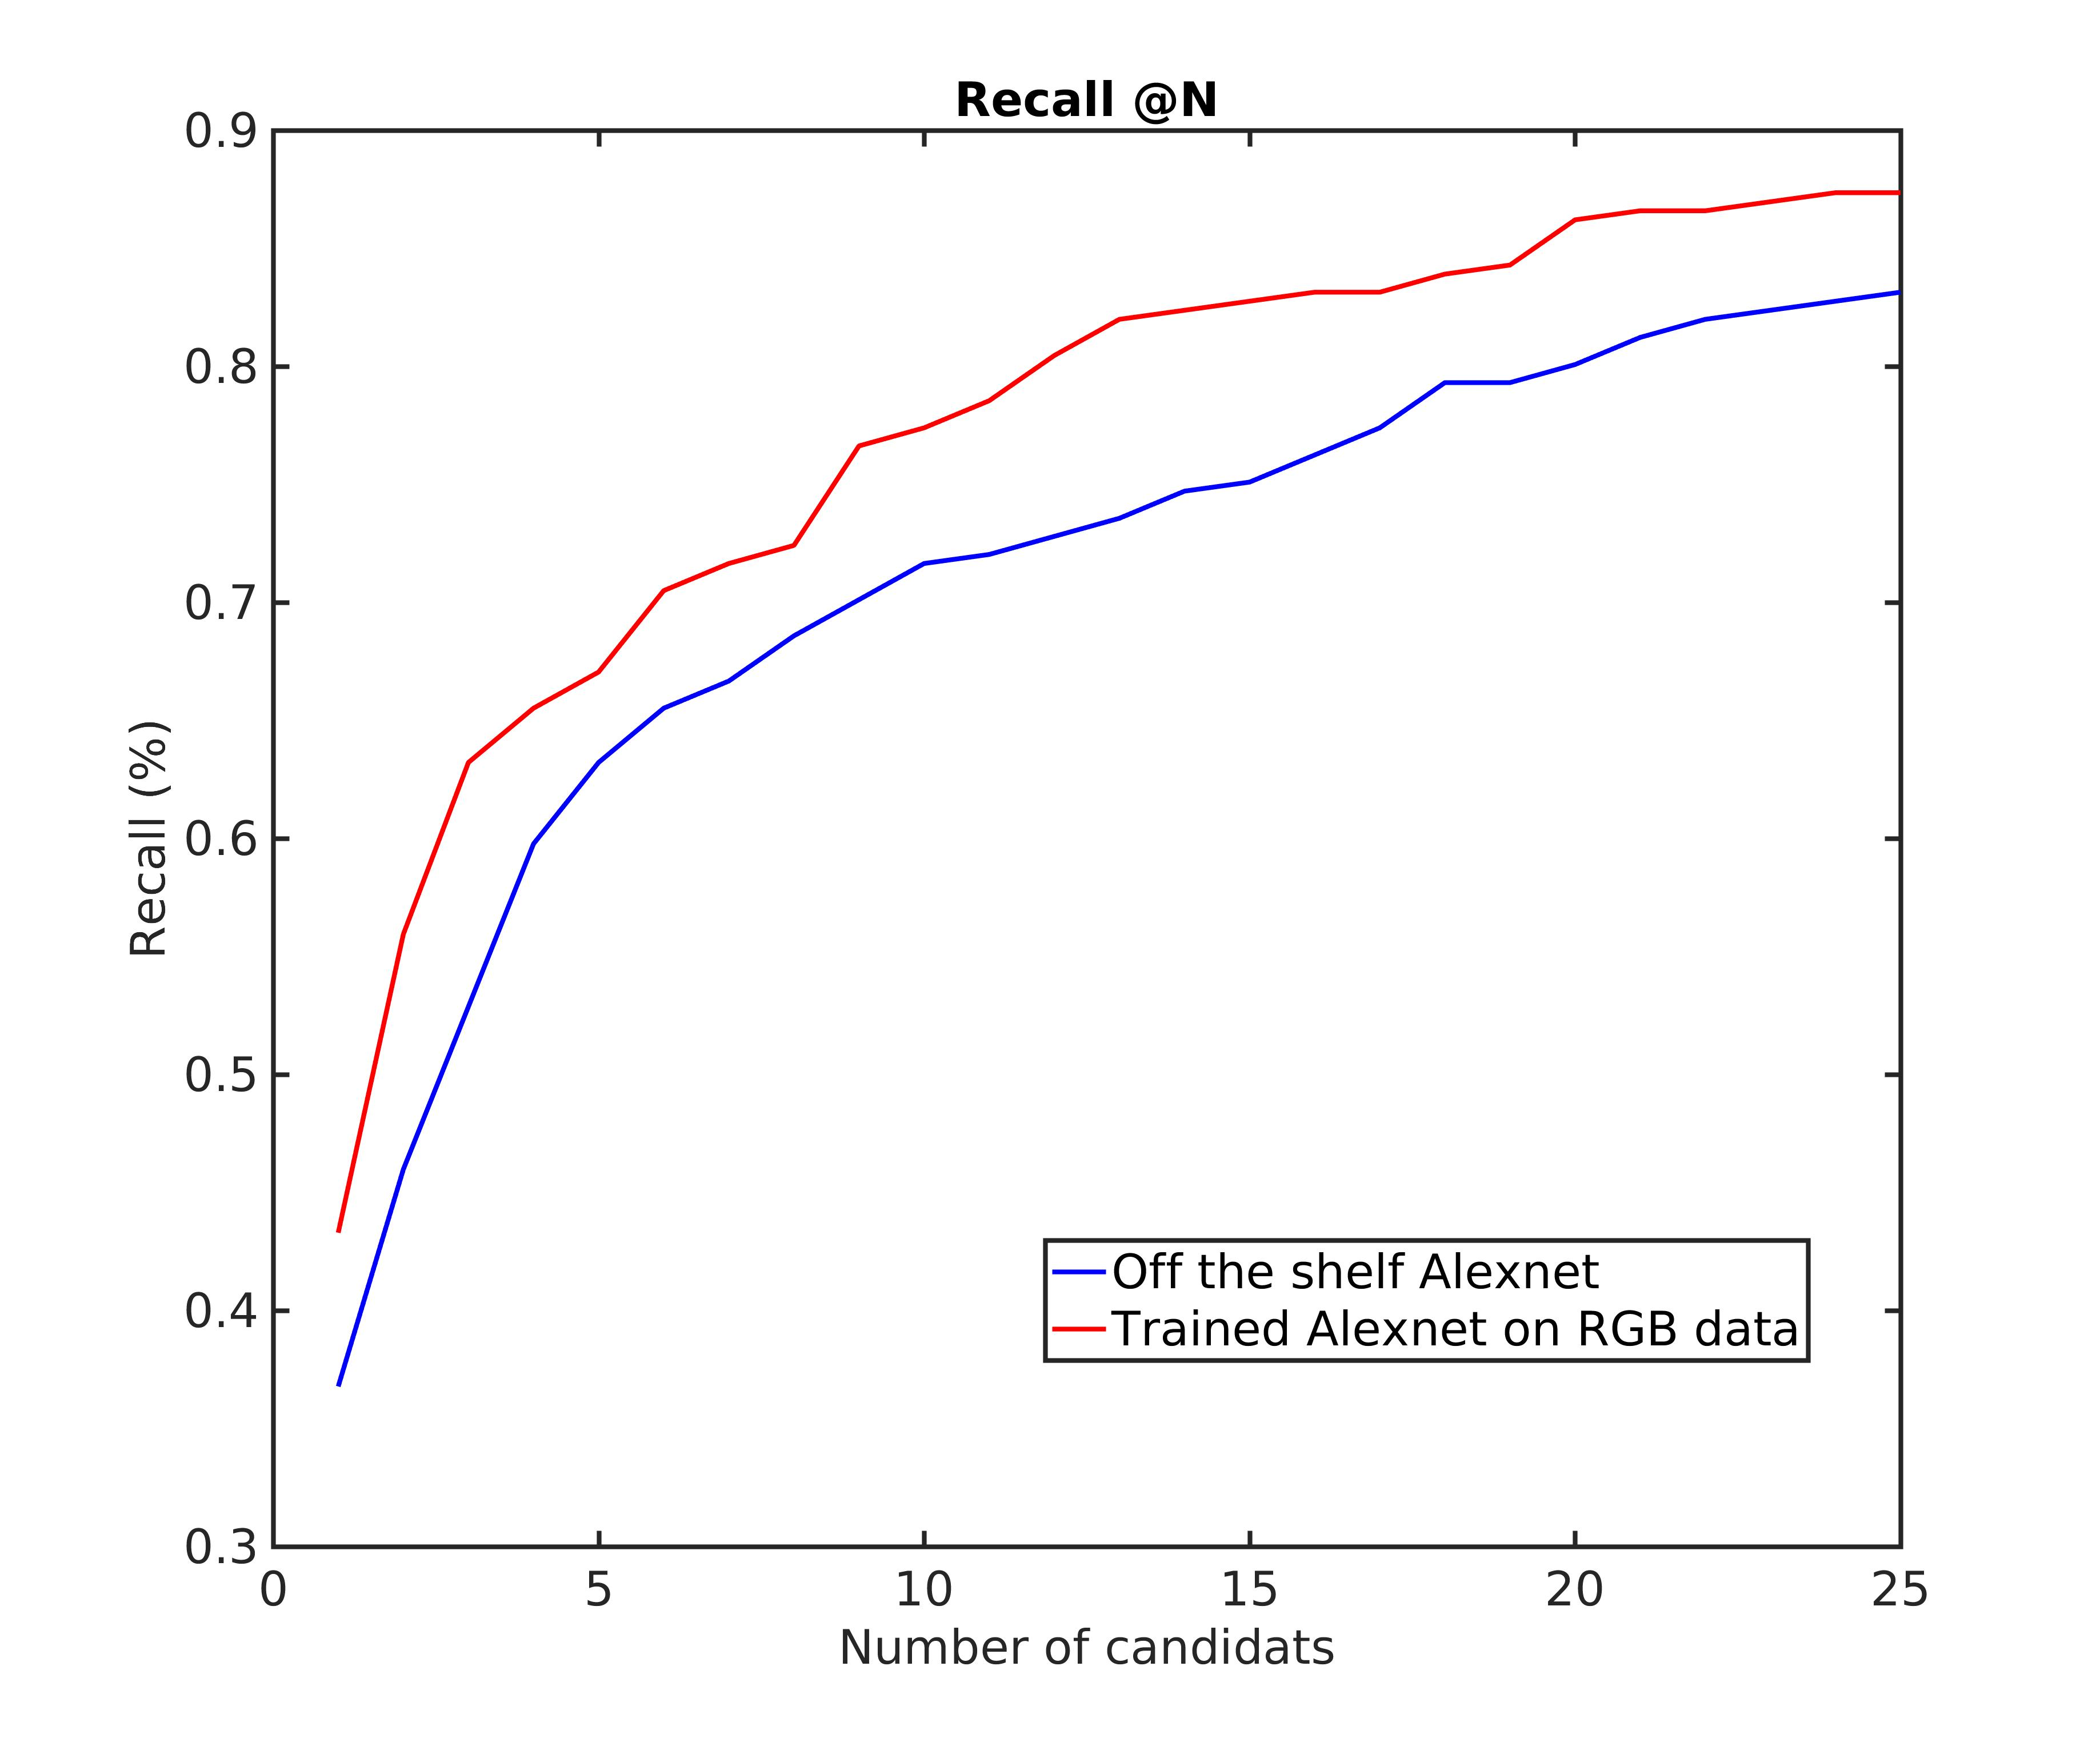
\includegraphics[width=0.5\linewidth]{images/result.jpg}	
	\end{figure}
	\vfill
	First results \textbf{are not} better with our Encoder-Decoder net than results obtained with single Encoder training.
\end{frame}